\documentclass[conference]{IEEEtran}

% ===== Packages =====
\usepackage{graphicx}
\usepackage{amsmath}
\usepackage{siunitx}
\usepackage{cite}
\usepackage{tikz}
\usetikzlibrary{arrows.meta,positioning,fit,calc,shapes.geometric,decorations.pathreplacing}
\usepackage[hidelinks]{hyperref}
\urlstyle{same}

% ===== Title & Author =====
\title{Lead-free Bio-Inkjet Printing with Bulk KNN Actuators and AITL-based Adaptive Control}

\author{
  \IEEEauthorblockN{Shinichi Samizo}
  \IEEEauthorblockA{Independent Semiconductor Researcher\\
  Former Engineer at Seiko Epson Corporation\\
  Email: \href{mailto:shin3t72@gmail.com}{shin3t72@gmail.com}\\
  GitHub: \url{https://github.com/Samizo-AITL}}
}

\begin{document}
\maketitle

% ===== Abstract =====
\begin{abstract}
This paper proposes a biocompatible inkjet printing architecture based on
lead-free piezoelectric actuators, specifically bulk KNN (K,Na)NbO$_3$, combined
with chip-on-film (COF) driver ICs, silicon cavity integration, and
an AITL (Adaptive Intelligent Three-Layer) supervisory control framework.
Unlike conventional PZT-driven industrial heads, the KNN approach supports
biocompatibility and Pb-free compliance, while moderate performance
(3--5 pL droplets, $10^6$ shots, $\pm50$ V operation) satisfies bioprinting needs.
Beyond actuation, the electromechanical response of KNN is leveraged for
\emph{self-diagnosis}: detecting missing droplets and estimating ink viscosity.
This diagnostic data feeds into an AITL architecture---an inner PID loop for
real-time stability, an FSM layer for mode transitions and compensation,
and an LLM-driven supervisory layer for adaptive redesign of control rules.
We present the architecture, process flow, and representative biomedical
applications, highlighting the potential of KNN as both actuator and sensor.
\end{abstract}

% ===== Sections =====
\section{Introduction}
\section{Introduction}

In the late 1990s, Japan's semiconductor industry was in transition. At Epson's Sakata 8-inch fab, DRAM was \emph{not} pursued as an end business; rather, DRAM technology transfer was used as a \textbf{strategic vehicle} to absorb submicron process technologies at and beyond 0.35~\si{\micro\meter} and redeploy them into Epson's core devices (ASICs, logic ICs, display drivers, and inkjet driver ICs).

The technology transfer from Mitsubishi covered three nodes, each with a clear role:
(1) 0.5~\si{\micro\meter} 16~Mbit DRAM --- to establish mass-production capability and stabilize fab operation; 
(2) 0.35~\si{\micro\meter} 64~Mbit DRAM (2nd gen) --- to introduce a scaled process while tackling yield window narrowing; 
(3) 0.25~\si{\micro\meter} 64~Mbit DRAM (3rd gen) --- as the next-stage validation bed and the basis for in-house deployment.

This paper focuses on the 0.25~\si{\micro\meter} (3rd gen) ramp-up in 1998: a process overview, the ramp-up method, and a failure-analysis–driven yield-improvement cycle. We also trace how these results enabled the 0.25~\si{\micro\meter} mobile pseudo-SRAM (VSRAM) in 2001 and why trench-based 0.18~\si{\micro\meter} VSRAM was abandoned.


\section{Background: Pb-free Piezoelectrics}
We summarize cell/circuit features of the 0.25-\textmu m 64-Mbit DRAM (stack capacitor, divided word-line, WSi stacks), and the wafer-test binning (Bin1--Bin7). For VSRAM, SRAM-like access is achieved by internal refresh logic while keeping DRAM cells; mobile-grade operation extended the temperature guarantee from 80~\si{\celsius} to 90~\si{\celsius}.


\section{Proposed Bio-IJ Architecture}
The associated \textit{process flow} begins with fabrication of the bulk
KNN stack and electrode finishing, followed by terminal cutting and COF
assembly. The actuator is then mounted with a heat spreader for thermal
management and finally bonded to the silicon cavity structure,
resulting in an integrated Bio-IJ printhead module.

% ===== Figures =====
\begin{figure}[t]
  \centering
  % TODO: Replace with TikZ or external PDF/PNG
  \includegraphics[width=0.9\linewidth]{figures/block_diagram.pdf}
  \caption{System architecture of the proposed Bio-Inkjet (Bio-IJ).
  The design integrates a bulk KNN multilayer actuator, COF driver IC,
  silicon cavity/nozzle array, and fluidic components (reservoir with
  PI damper and back-pressure control).}
  \label{fig:block}
\end{figure}

\begin{figure}[t]
  \centering
  % TODO: Replace with TikZ or external PDF/PNG
  \includegraphics[width=0.9\linewidth]{figures/cross_section.pdf}
  \caption{Cross-sectional schematic of the Bio-IJ printhead.
  The bulk KNN actuator is bonded onto a silicon cavity with outlet
  nozzles of $\varphi$\SI{8}{\micro\meter}, supported by reservoir
  fluidics, damping, and back-pressure stabilization.}
  \label{fig:section}
\end{figure}


\section{Self-Diagnosis and Feedback Control}
The bulk KNN actuator can also function as a proxy sensor by monitoring
its electromechanical response during drive pulses.
\subsection{Dot-Missing Detection and Compensation}
By observing charge/displacement signatures, missing droplets are detected
without external optics. An FSM controller triggers neighboring-nozzle
compensation, preserving array-level print reliability.
\subsection{Viscosity Estimation and Drive Adaptation}
Viscosity changes appear as altered dynamic response.
The PID loop adjusts drive voltage/pulsewidth in real time.
This closes the loop between fluid rheology and actuator operation.

\section{AITL Control Framework}
The Adaptive Intelligent Three-Layer (AITL) framework integrates:
\begin{itemize}
\item \textbf{Inner PID}: ensures real-time stability of droplet ejection.
\item \textbf{Intermediate FSM}: supervises nozzle states, detects anomalies,
and switches modes (normal, compensation, cleaning).
\item \textbf{Outer LLM}: analyzes long-term trends, re-identifies PID gains,
and redefines FSM transitions when performance degrades.
\end{itemize}
A schematic is shown in Fig.~\ref{fig:aitl}.
\begin{figure}[t]
\centering
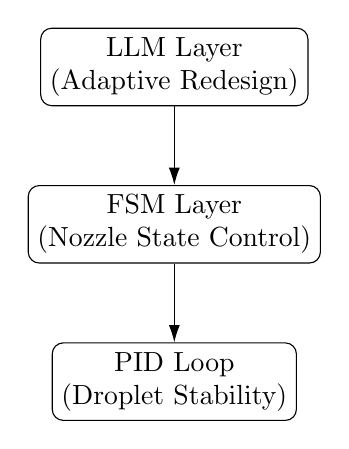
\begin{tikzpicture}[
  block/.style={draw, rounded corners, minimum width=2.4cm, minimum height=8mm, align=center},
  line/.style={-{Latex[length=2.2mm,width=1.4mm]}}
]
\node[block] (pid) {PID Loop\\(Droplet Stability)};
\node[block, above=of pid] (fsm) {FSM Layer\\(Nozzle State Control)};
\node[block, above=of fsm] (llm) {LLM Layer\\(Adaptive Redesign)};
\draw[line] (fsm) -- (pid);
\draw[line] (llm) -- (fsm);
\end{tikzpicture}
\caption{AITL three-layer architecture for Bio-IJ adaptive control.}
\label{fig:aitl}
\end{figure}

\section{Applications}
\section{Applications}
Potential applications include:
\begin{itemize}
  \item \textbf{Cell patterning}: deposition of living cells with survival rates above 80\%.
  \item \textbf{Protein microarrays}: picoliter deposition of antibodies or DNA spots.
  \item \textbf{Hydrogel 3D printing}: pL-scale deposition followed by UV or thermal curing.
\end{itemize}

The moderate performance of KNN actuators is sufficient for these
applications, where droplet volume control and biocompatibility are
more critical than long-term durability.


\section{Conclusion}
\section{Conclusion}
This paper has proposed a Bio-Inkjet (Bio-IJ) architecture based on
bulk KNN actuators as a lead-free alternative to conventional PZT-based
printheads.
By combining multilayer KNN stacks, COF driver ICs, and silicon cavity
integration, the system achieves picoliter-scale droplet generation
under moderate voltages while ensuring material biocompatibility.

Unlike industrial printing, where full PZT compatibility in terms of
maximum $d_{33}$, billion-cycle endurance, and cost efficiency is
required, biomedical printing places emphasis on safety, controlled
droplet volume, and operational reliability over shorter lifetimes.
The proposed approach aligns well with these requirements, providing
sufficient performance for applications such as cell patterning,
protein microarrays, and hydrogel 3D fabrication.

These findings highlight bulk KNN as a practical foundation for
standardizing lead-free Bio-IJ systems in research, clinical, and
educational domains.
Future work will involve experimental validation of droplet formation,
long-term reliability testing under bio-relevant conditions, and system
integration with existing bioprinting workflows.

\textbf{Most importantly, this work emphasizes that in biomedical inkjet
printing, safety and biocompatibility must take precedence over extreme
performance metrics, positioning KNN-based Bio-IJ as a safe and viable
path toward Pb-free bioprinting.}


% ===== References =====
\nocite{Saito2004KNN,Dubois2019BioIJ}
\bibliographystyle{IEEEtran}
\bibliography{refs}

% ===== Biography =====
\section*{Author Biography}
\textbf{Shinichi Samizo} received the M.S. degree in Electrical and Electronic
Engineering from Shinshu University, Japan. He worked at Seiko Epson
Corporation as an engineer in semiconductor memory and mixed-signal
device development, and contributed to inkjet MEMS actuators and
PrecisionCore printhead technology. He is currently an independent
semiconductor researcher focusing on process/device education, memory
architecture, and AI system integration. Contact:
\href{mailto:shin3t72@gmail.com}{shin3t72@gmail.com}.
\end{document}
